%%%%%%%%%%%%%%%%%%%%%%%%%%%%%% -*- Mode: Latex -*- %%%%%%%%%%%%%%%%%%%%%%%%%%%%
%% project.tex -- 
%% Author          : Philip Johnson
%% Created On      : Tue Nov  4 10:26:48 1997
%% Last Modified By: Philip M. Johnson
%% Last Modified On: Mon Jun 13 16:20:21 2005
%% RCS: $Id$
%%%%%%%%%%%%%%%%%%%%%%%%%%%%%%%%%%%%%%%%%%%%%%%%%%%%%%%%%%%%%%%%%%%%%%%%%%%%%%%
%%   Copyright (C) 1997 Philip Johnson
%%%%%%%%%%%%%%%%%%%%%%%%%%%%%%%%%%%%%%%%%%%%%%%%%%%%%%%%%%%%%%%%%%%%%%%%%%%%%%%
%% 

\section{Overview}

\subsection{Motivation}
As with baseball, physics, music, and other skillful human endeavors, there
is a vast range of ability associated with software development.  For
almost 40 years, software development researchers have been attempting to
understand, measure, and support the development of superior skill in
software development.  Sackman performed the seminal research on programmer
productivity in 1967, in which he reported a 28:1 difference between the
slowest and fastest programmers on a programming task \cite{Sackman68}.
Subsequent research by Prechelt on Sackman's original dataset in
combination with other published datasets indicates a smaller but still
significant multiple---from 2:1 to 6:1 depending upon conditions and the
kind of statistical comparison used \cite{Prechelt99}.

While comparison of different programmer's effort on a common task is the
most direct way to detect productivity variability, it is not the only way.
One alternative  employs the COCOMO II cost estimation model
\cite{Boehm00}. COCOMO uses a dataset of approximately 160 completed
industrial projects to calibrate a model that computes the effort required
to complete a project based upon characteristics of the software to be
developed and the organization doing the development.  In COCOMO, the
effort differential between best and worst programming teams with respect
to capability is 3.53, applications experience is 1.51, language and tools
experience is 1.43, platform experience is 1.40, and team cohesion is 1.29.
Multiply these together, and the COCOMO model indicates a theoretical
productivity difference of 13:1 between the most suited and least suited
programming teams for a given software project. 

Of course, one can also argue that there is infinite variability between
programmers, since certain kinds of programming tasks are so challenging
that some programmers will never complete them no matter how much effort
they invest. For example, in a private correspondence with a former member
of a tool development team for a major vendor, he stated that he viewed his
product as inferior to a competitor's and that it would most likely would
remain so regardless of the level of resources expended by his company,
basically because the competitor's product development was led by a world
class designer.  In summary, while the actual multiple can be debated, the
presence of substantial programmer variability cannot.


Programmer variability creates two basic kinds of challenges for the
software engineering research community: (1) How can we raise the average
productivity of software developers, and (2) How can we reduce the
variability between the best and worst software developers?  In general, we
have responded to these challenges in one or more of three ways: through
abstraction, automation, or best practices.

The evolution of programming languages from machine language to assembly
language to high level languages to executable specification languages
exemplifies the successful application of abstraction to improving the
average productivity of software developers by reducing the amount and
complexity of code required to accomplish a given task.  A single keyword
such as ``synchronized'' in a high level language like Java might require
thousands of lines of code to implement correctly in assembly language.
Indeed, software disasters such as the Therac-25 were ultimately
attributed to incorrect implementation of synchronization in custom
software in a low-level language \cite{Leveson93}.

Automation refers to the development of scripts or other approaches to
ensuring that a sequence of development tasks are carried out consistently,
reliably, and correctly.  One example is an automated daily build
mechanism, which might (a) create a ``clean'' initial build state, (b)
check out the latest version of a system from a configuration management
repository, (c) compile the latest version, (d) deploy the latest version
to a run-time environment (such as installation on a web server), (e) run
all functional (i.e. unit) and non-functional (i.e. load) tests associated
with the latest version, (g) build the documentation associated with the
latest version, (h) generate a report associated with the build process,
and (i) email results to developers and managers.  

The difference between abstraction and automation is that abstraction
creates a ``black box'' while automation does not. For example, the
implementation of the synchronized keyword in Java is a black box: no
application developer would be expected to maintain or debug this language
construct and, in general, developers can simply assume that this
abstraction functions correctly.  A daily build script which is developed,
debugged, and maintained by developers does not provide abstraction but
nevertheless provides important benefits as a form of automation: it can
vastly reduce the productivity impact of developers not carrying out the
sequence of actions required to build the product correctly, or even the
productivity impact of not building the system at all due to the time,
overhead, and tedium associated with the activities.

While abstraction is the province of languages and other expressive media,
and automation is the province of tools and environments, best practices
focus on the behavior and activities of people during software development.
The seminal software engineering best practice is the waterfall lifecycle
model, which was first described in the early 1970's and provided an
efficient and effective partitioning of development into a sequence of
phases: specification, design, implementation, testing, and maintenance.
Provided that system requirements can be specified in advance and are
guaranteed not to change, the waterfall lifecycle model still constitutes a
viable best practice for software engineering.

The Software Engineering Body of Knowledge (SWEBOK) illustrates the variety
of forms of best practice \cite{Abran05}.  SWEBOK provides a map to the
state of the art in software engineering, and divides the landscape into
ten areas: requirements, design, construction, testing, maintenance,
engineering management, configuration management, process, tools, and
quality.  The SWEBOK material shows that abstraction, automation, and best
practices are not independent concepts but are instead deeply entwined:
best practices (such as testing) engender new forms of abstraction (formal
languages for testing) and automation (tools for automated test definition
and/or invocation). Conversely, new tools (such as automated test
frameworks) can catalyze new best practices (such as test driven design).

One might naively assume that becoming a world class software development
group would require nothing more than downloading the SWEBOK and
implementing all of its best practices and the abstractions and automations
that they require.  Unfortunately, software engineering best practices are
highly contextual: a practice that provides immense benefits in one
organizational culture and development context could prove disastrous in
another. For example, a best practice such as Cleanroom might be essential
in the development of a complex, life-critical application but too costly
to justify in a startup environment where time to market is critical.  In
addition, software engineering best practices can be in conflict.  The
Extreme Programming \cite{Beck00} best practice eschews the use of the Code
Inspection \cite{Fagan76} best practice, claiming that the use of Pair
Programming obviates the need for a separate inspection activity.

The context sensitivity of software engineering best practices creates a
number of problems. First, how can an organization improve by adoption of
best practices when it is so difficult to determine their appropriateness?
Some organizations might address this problem via a trial-and-error
approach, where various best practices are ``tried on for size''.  Others
might hire consultants to tell the organization which practices to
adopt. Still others might utilize models for process improvement such as
the CMMI \cite{Royce02}, which could be viewed as ``best practices for
adopting best practices''.

Second, how do ``best practices'' actually become recognized as such?  For
example, the best practice of ``Extreme Programming'' would likely have
become a forgotten experiment in an alternative software development
process at Chrysler Corporation had Kent Beck not decided to vigorously
market the approach with books, lectures, and networking.  Ironically, the
project on which XP based its initial claims for success was eventually
canceled without fulfilling its requirements and is now used as evidence
against XP by its detractors \cite{Keefer03}.

In summary, software engineering uses three methods to address the problem
of programmer productivity variability: abstraction, automation, and best
practices.  Unfortunately, the creation of best practices, and their
adoption into new contexts is traditionally mediated by political and
social processes that may be quite unrelated to the actual effectiveness of
the practice and its associated abstractions/automations in the 
organization.


\subsection{Approach}

This research proposal presents a new, evidence-based approach to the
generation and adoption of best practices.  Instead of looking outward into
the community for best practices, and attempting to adapt them to one's own
environment, our research will investigate how best practices can emerge
organically from within one's current organizational and project context.
Instead of relying on politics or persuasiveness for adoption, our research
approach involves instrumentation that generates empirical data that can be
used to either argue for the benefits of adoption, or else provide evidence
that the practice is not actually effective in the current context.
Finally, our research will involve analytic approaches designed to generate
candidate best practices from data mining techniques applied to process and
product data.

This research approach is made possible by our research and development
activities over the past four years in Project Hackystat \cite{Hackystat}, an open source
framework for automated collection and analysis of software engineering
process and product data.  The Hackystat system provides a unique
technological and methodological foundation that we will leverage to pursue
this research.  First, Hackystat implements an automated approach to
metrics collection by attaching sensors to development tools. This makes it
possible to capture both low and high-level data about processes and
products with a level of precision and completeness not possible with
manual approaches. Second, Hackystat provides an implementation of Software
Project Telemetry, an approach to in-process monitoring, analysis, and
decision-making based upon the generation of high-level abstractions of the
sensor data stream.  Software Project Telemetry provides a means to
understand whether the overall project trajectory is stable, improving, or
declining at a particular point in time. Third, Hackystat provides a prototype
implementation of Software Development Stream Analysis, which observes the
low-level behaviors (i.e.  practices) of individuals and classifies them in
various ways. For example, SDSA can be used to identify when a developer is
using test-driven design.

The combination of Hackystat, Software Project Telemetry, and Software
Development Stream Analysis provide a mechanism for emergent,
context-sensitive evaluation of best practices within an organization.  For
example, an organization using Hackystat on a project can use Software
Project Telemetry to establish baseline values for various software
development measures.  Software Development Stream Analysis provides a way
to characterize the practices of developers as they perform development
activities.  Integrating these two analyses together provides a way to
relate the practices of developers to their outcomes in terms of process
and product measures. So, for example, if a developer decides to switch to
the use of pair programming on a trial basis, they can see if this new
practice makes an impact on the measures of process and product captured by
Software Project Telemetry.  Conversely, if Software Project Telemetry
reveals a significant decline in process or product metrics (such as a drop
in the test case coverage of the system), the Software Development Stream
Analyses can be used to assess whether some change in practice could be
responsible (such as a change from test-first to test-last design).

Hackystat, Software Project Telemetry, and Software Development Stream
Analysis together form an empirical, low-cost, and in-process approach to
assessing best practices when the practices are known a priori and
recognition rules for them can be built into the SDSA system.  The final
component of this research will investigate approaches to the discovery of
new best practices.  To do this, we will incorporate recent research in data
mining known as ``episode discovery'' \cite{Heierman04,Mannila95,Agrawal95}.  The
goal of episode discovery is to uncover behavioral patterns in a stream of
time-stamped data.  For example, in a ``smart house'', if an occupant
repeatedly turns on a light after opening the front door, the episode
discovery mechanism should discover this pattern after a number of
repetitions, thus enabling the smart house to begin automatically turning
on the light whenever the front door is opened by this occupant.  In this
research, we will use episode discovery to uncover repeated patterns in
developer behavior, and correlate them to the software project telemetry
data.  As a simple example, episode discovery might find that one developer
consistently writes and executes tests against their code prior to
committing it to the CVS repository, and that this pattern is correlated
with significantly less daily build failures attributed to this developer.

Our approach compares in interesting ways to more traditional approaches to
evaluation of best practices, which involve the trial adoption of the best
practice, the collection of data on the effect of the practice, and an
eventual assessment of efficacy of the practice.  While our approach
mirrors the tradition at this level, it differs radically in the social and
organizational context surrounding the evaluation.  Rather than best
practice evaluation being a ``one off'' experiment, it becomes a
continuous, embedded aspect of an ongoing software development project.
Rather than traditional evaluation approaches, in which the development
project is fully completed in order to gather outcome values of use to
assessment, our approach uses software project telemetry, which allows
ongoing, in-process analysis over the course of a project.  Finally, our approach
investigates the use of data mining techniques to uncover new best
practices.  

\subsection{Objectives}

The overall objective of this research is to design, implement, and
evaluate a continuous, evidence-based approach to in-process discovery and
assessment of context-sensitive best practices during software development.
This overall objective has the following sub-objectives: 

\begin{itemize}
  
\item Enhancement of the Software Development Stream Analysis mechanism to
  support a variety of current best practices, and determination of the
  kinds of best practices that are amenable (or not amenable) to
  recognition using SDSA.

\item Development of integration mechanisms between SDSA and Software
  Project Telemetry in order to allow users to determine how practices
  recognized by SDSA relate to telemetry data any particular point in time.
  
\item Development of an episode discovery subsystem in Hackystat to support
  automated recognition of patterns in developer behavior.
  
\item Classroom-based, case study evaluation of the proposed techniques. In
  addition to providing initial data regarding the effectiveness of our
  approach, classroom use will help us to refine the technology, develop
  curriculum materials, and ready the approach for industrial evaluation.
  
\item Industry-based evaluation of the proposed techniques. Following
  classroom evaluation, we will embark on at least one industry case study
  with the goal of assessing the suitability of this technique in a
  ``real-world'' environment.
  
\item Packaging of the system and methods for widespread dissemination. We
  will continue the process we have followed with the Hackystat Project of
  making our technology and results continuously available to the software
  engineering community through frequent stable releases of the system and
  read-only access to our CVS repositories for the latest changes.  
  
\item Development of curriculum materials regarding continuous,
  evidence-based discovery and assessment of software engineering best
  practices. As with Hackystat, we will develop software engineering
  curriculum materials and assignments that enable the study and analysis
  of this approach in academic settings.

\end{itemize}


\section{Related Work}

\subsection{Evidence-based software engineering}

A recent revolution in medical research involves the introduction of an
``evidence-based'' paradigm.  This paradigm arose in response to two
observations: the failure to organize medical research into systematic
reviews could cost lives, and the clinical judgment of experts compared
unfavorably with the results of systematic reviews.   The evidence-based 
approach is starting to be applied outside of medicine, in fields such as
psychiatry, nursing, social policy, education, and software engineering. 

Kitchenham has been leading the movement for evidence-based software
engineering, organizing workshops on this topic and publishing papers
explaining the issues involved in applying evidence-based research
techniques to software engineering \cite{Kitchenham04,Kitchenham04a}.  She
and her collaborators propose a five step method for evidence-based
software engineering: (1) Convert the need for information [about a
software engineering practice] into an answerable question; (2) Track down
the best evidence available for answering the question; (3) Critically
appraise that evidence for its validity (closeness to the truth), impact
(size of the effect), and applicability (usefulness in software development
practice); (4) Integrate the critical appraisal with current software
engineering knowledge and stakeholder values [to support decision-making];
(5) Evaluate the effectiveness and efficiency in applying Steps 1-4 and
seek ways to improve them for next time.  While promising, application of 
systematic reviews and the integration of empirical software engineering data
from multiple sources has been found to be challenging \cite{Jedlitschka04}.



\subsection{Hackystat}

For the past several years, we have been developing a framework for
automated software development process and product metric collection
and analysis called Hackystat.  This framework differs from other
approaches to automated support for product and process measurement in
one or more of the following ways:

\begin{itemize}

\item Hackystat uses sensors to unobtrusively collect data from development
environment tools; there is no chronic overhead on developers to collect
product and process data.

\item Hackystat is tool, environment, process, and application agnostic.
The architecture does not suppose a specific operating system platform, a
specific integrated development environment, a specific software process,
or specific application area.  A Hackystat system is configured from a set
of modules that determine what tools are supported, what data is collected,
and what analyses are run on this data.

\item Hackystat is intended to provide in-process project management
support. Many traditional software metrics approaches are based upon the
``project repository" method, in which data from prior completed projects
are used to make predictions about or support control of a current
project. In contrast, Hackystat is designed to collect data from a current,
ongoing project, and use that data as feedback into the current project.

\item Hackystat provides infrastructure for empirical experimentation.  For
those wishing to compare alternative approaches to development, or for
those wishing to do longitudinal studies over time, Hackystat can provide a
low-cost approach to gathering certain forms of project data.

\item Hackystat is open source and is available to the academic and
commercial software development community for no charge.

\end{itemize}

The design of Hackystat \cite{csdl2-02-07} has resulted from of prior
research in our lab on software measurement, beginning with research into
data quality problems with the PSP \cite{csdl-98-11} and which
continued with the LEAP system for lightweight, empirical, anti-measurement
dysfunction, and portable software measurement
\cite{csdl2-00-03}.

\begin{figure*}[htpb]
  \centering
  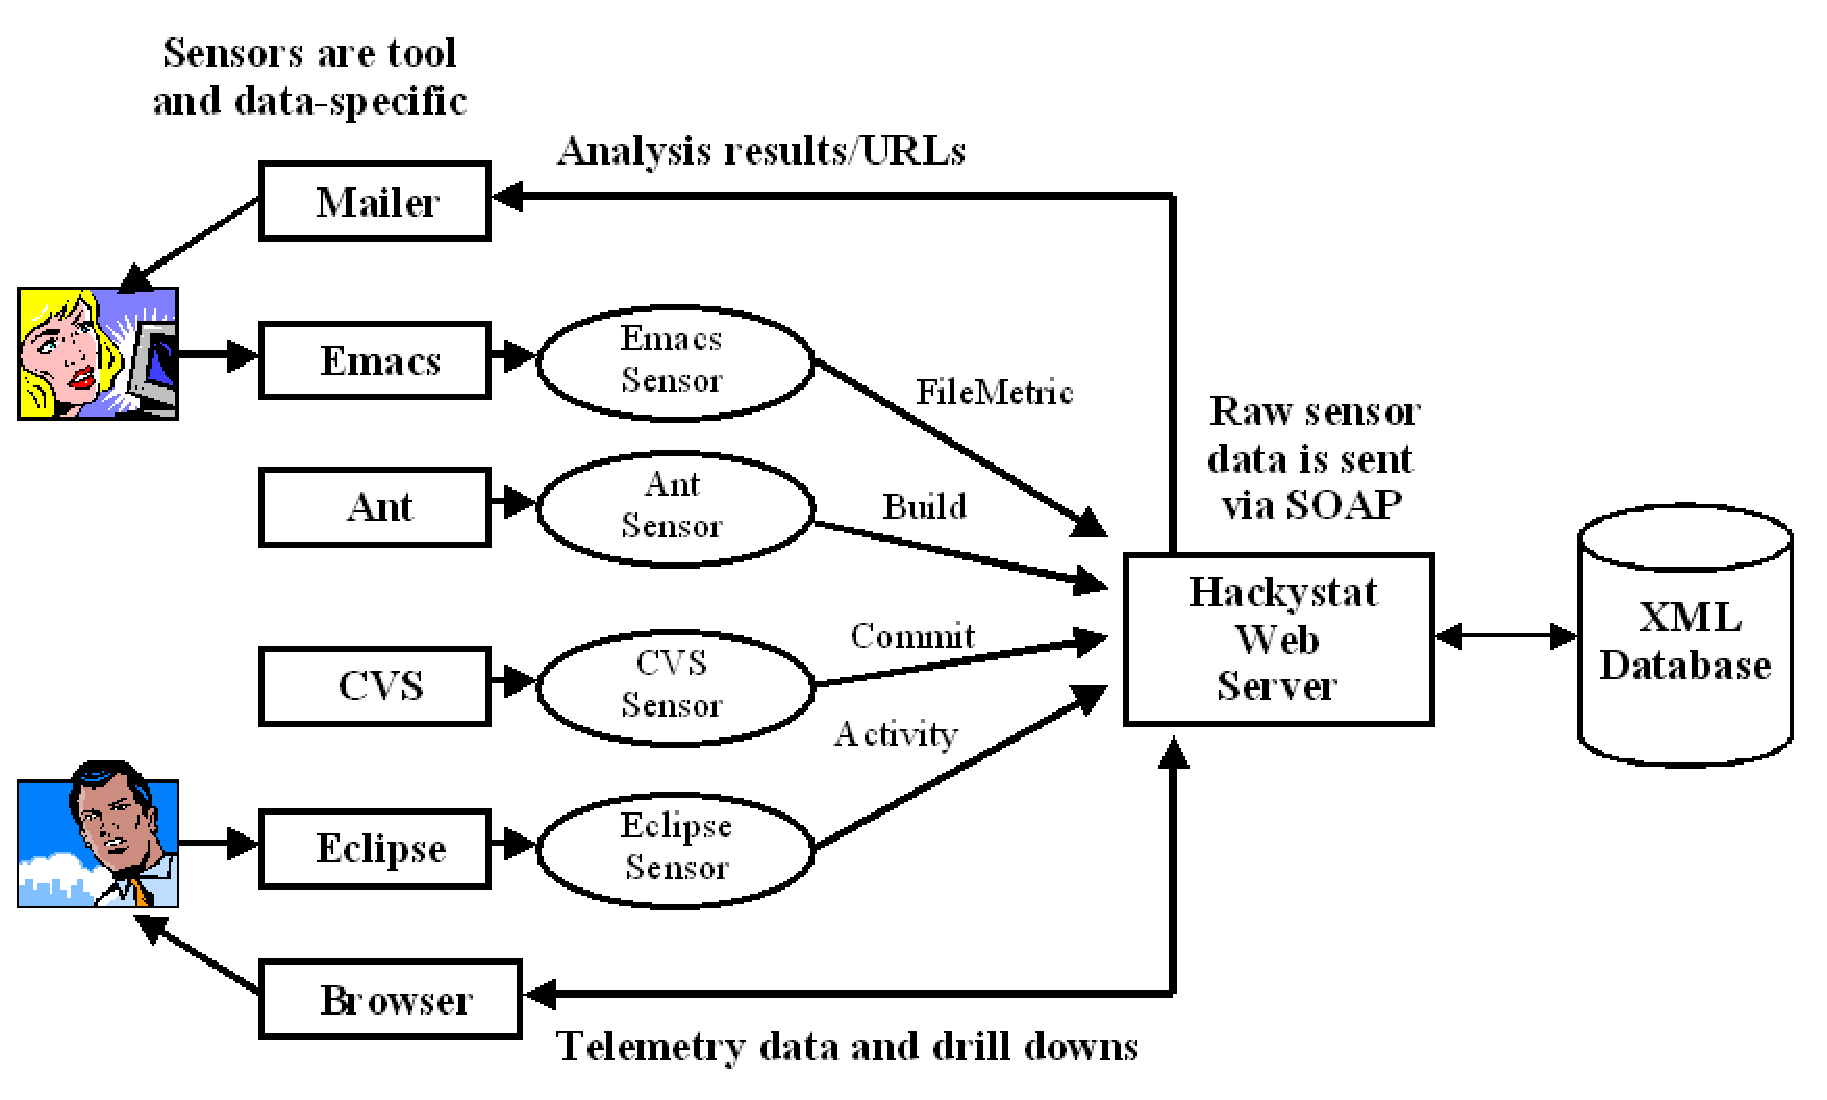
\includegraphics[width=0.60\textwidth]{architecture.eps}
  \caption{The basic architecture of Hackystat. Sensors are attached to
  tools directly invoked by developers (such as Eclipse or Emacs) as
  well as to tools implicitly manipulated by developers (such as CVS or 
  an automated build process using Ant).}
  \label{fig:architecture}
\end{figure*}

To use Hackystat, the project development environment is 
instrumented by installing Hackystat sensors, which developers attach
to the various tools such as their editor, build system, configuration
management system, and so forth. Once installed, the Hackystat sensors
unobtrusively monitor development activities and send process and
product data to a centralized web service.  If a user is working
offline, sensor data is written to a local log file to be sent
when connectivity can be established with the centralized web service.
Project members can then log in to the web server to see the collected
raw data and run analyses that integrate and abstract the raw sensor
data streams into telemetry.  Hackystat also allows project members to
configure ``alerts`` that watch for specific conditions in the
sensor data stream and send email when these conditions occur. Figure
\ref{fig:architecture} illustrates the basic architecture of the system. 

Hackystat is an open source project. Its  sources, binaries, and
documentation are available at http://www.hackystat.org.  There is also a
public server available at http://hackystat.ics.hawaii.edu.  Hackystat has
been under active development for approximately four years, and currently
consists of approximately 1500 classes and 95,000 lines of code.  Sensors are
available for a variety of tools including Eclipse, Emacs, JBuilder,
Jupiter, Jira, Visual Studio, Ant, JUnit, JBlanket, CCCC, DependencyFinder,
Harvest, LOCC, Office, and CVS.  

\subsection {Software Project Telemetry}
\label{sec:telemetry}

A major application of Hackystat has been the development of a new
approach to software measurement analysis called ``Software Project
Telemetry``. We define Software Project Telemetry as a style of
software engineering process and product collection and analysis which
satisfies the following properties:

{\em Software project telemetry data is collected automatically by tools
that unobtrusively monitor some form of state in the project development
environment.}  In other words, the software developers are working in a
``remote or inaccessible location`` from the perspective of metrics
collection activities. This contrasts with software metrics data that
requires human intervention or developer effort to collect, such as PSP/TSP
metrics \cite{Humphrey95}.
        
{\em Software project telemetry data consists of a stream of time-stamped
events, where the time-stamp is significant for analysis.}  Software
project telemetry data is thus focused on evolutionary processes in
development.  This contrasts, for example, with COCOMO \cite{Boehm00},
where the time at which the calibration data was collected about the
project is not significant.

{\em Software project telemetry data is continuously and immediately
available to both developers and managers.}  Telemetry data is not hidden
away in some obscure database guarded by the software quality improvement
group.  It is easily visible to all members of the project for
interpretation.

{\em Software project telemetry exhibits graceful degradation.}  While
complete telemetry data provides the best support for project management,
the analyses should not be brittle: they should still provide value even if
sensor data occasionally ``drops out`` during the project. Telemetry
collection and analysis should provide decision-making value even if these
activities start midway through a project.
         
{\em Software project telemetry is used for in-process monitoring, control,
and short-term prediction.} Telemetry analyses provide representations of
current project state and how it is changing at the time scales of days,
weeks, or months.  The simultaneous display of multiple project state
values and how they change over the same time periods allow opportunistic
analyses---the emergent knowledge that one state variable appears to
co-vary with another in the context of the current project.

Software Project Telemetry enables a more incremental, distributed,
visible, and experiential approach to project decision-making. It also
creates perspectives on system development that can provide new insight
into HPC development processes, as we illustrate in the case study below.


\subsection{Software Development Stream Analysis}

Zorro is built on top of Hackystat platform. Development activity data is
grouped together for development streaming, stream tokenization and episode
classification. Development stream is divided into small episodes with the
help of tokenizer. Each episode is a series of continuous activities that
are isolated by token activities. For instance, test-pass episodes are
created when there is a successful unit test invocation. All development
activities happened between two continuous successful test invocations
belong to this test-pass episode. We evaluate episode with pre-defined
rules using JESS \cite{Friedman-Hill:03} rule engine system.


Hackystat sensors collect both process of software development and state
data of projects. To eclipse IDE sensor collects most development
activities such as new project, open project, new file, file open, file
close, file edit, refactoring, unit test etc. Same kind of activities
are grouped together to make sub development streams. They merge together to
make development stream. Activities
irrelevant to the project are filtered out in merging process.

\subsection{Episode Discovery}

Episode discovery related work goes here. 


\subsection{Results from prior NSF research}

\small
\begin{tabular}{lp{4.5in}}

Award number: & CCF02-34568 \\
Program: & Highly Dependable Computing and Communication Systems Research\\
Amount: & \$638,000 \\
Period of support: & September 2002 to September 2006 \\
Title of Project: & Supporting development of highly dependable software through
continuous, automated, in-process, and individualized software measurement validation \\
Principal Investigator: & Philip M. Johnson \\
Selected Publications: & \cite{csdl2-04-22,csdl2-04-13,csdl2-04-11,csdl2-03-12,csdl2-02-07,csdl2-03-07,csdl2-04-02,csdl2-04-04,csdl2-04-06}
\end{tabular} \\ %[3mm]
\normalsize

\medskip

The general objective of this research project is to design, implement, and
validate software measures within a development infrastructure that
supports the development of highly dependable software systems.
Contributions of this research project include: (a) development of a
specialized configuration of Hackystat to automatically acquire build and
workflow data from the configuration management system for the Mission Data
System (MDS) project at Jet Propulsion Laboratory; (b) development of
analyses over MDS build and workflow data to support identification of
potential bottlenecks and process validation; (c) identification of
previous unknown variation within the MDS development process; (d)
development of a generalized approach to in-process, continuous measurement
validation called ``Software Project Telemetry'', (e) substantial
enhancements to the open source Hackystat framework, improving its
generality and usability; (f) development of undergraduate and graduate
software engineering curriculum involving the use of Hackystat for
automated software engineering metrics collection and analysis; (g) support
for 3 Ph.D., 6 M.S., and 3 B.S. degree students. 



\section{Research Plan}



\section{Conclusions}
